% TEMPLATE for Usenix papers, specifically to meet requirements of
%  USENIX '05
% originally a template for producing IEEE-format articles using LaTeX.
%   written by Matthew Ward, CS Department, Worcester Polytechnic Institute.
% adapted by David Beazley for his excellent SWIG paper in Proceedings,
%   Tcl 96
% turned into a smartass generic template by De Clarke, with thanks to
%   both the above pioneers
% use at your own risk.  Complaints to /dev/null.
% make it two column with no page numbering, default is 10 point

% Munged by Fred Douglis <douglis@research.att.com> 10/97 to separate
% the .sty file from the LaTeX source template, so that people can
% more easily include the .sty file into an existing document.  Also
% changed to more closely follow the style guidelines as represented
% by the Word sample file. 

% Note that since 2010, USENIX does not require endnotes. If you want
% foot of page notes, don't include the endnotes package in the 
% usepackage command, below.

% This version uses the latex2e styles, not the very ancient 2.09 stuff.
\documentclass[letterpaper,twocolumn,10pt]{article}
\usepackage{usenix,epsfig,endnotes}
\usepackage[T1]{fontenc}
\usepackage{epstopdf}
\begin{document}

%don't want date printed
\date{}

%make title bold and 14 pt font (Latex default is non-bold, 16 pt)
\title{\Large \bf Building a Modular ROS Network for the Raven II}

%for single author (just remove % characters)
\author{
{\rm Troy\ Sankey}\\
University of California Los Angeles
\and
{\rm Qu\ (Jackie)\ Jin}\\
University of California Los Angeles
\and
{\rm Jonathan\ Chan}\\
University of California Los Angeles
} % end author


\twocolumn[
  \begin{@twocolumnfalse}
    \maketitle
    \vspace{5cm}
    \hfill
    \begin{minipage}{0.8\linewidth}
      \begin{abstract}

The Raven II Surgical Robot is a 7-DOF cable-actuated surgical robot
designed for minimally invasive and remote surgery. The robot can be
teleoperated with two Phantom Omnis which are haptic devices designed
for medical training and research applications. The Raven utilizes
Robot Operating System (ROS), a collection of software modules
specially made for developing robot applications. Many features of ROS
could be beneficial to the the Raven, but are inaccessible due to
current code's limited use of ROS constructs. The objective of our
team is to fully integrate ROS into the Raven II which would bring
better support for generic control, image processing, basic
automation, and overall cleaner and more reliable code. This report
covers the implementation of generic control based on ROS.

      \end{abstract}
    \end{minipage}
    \hfill
  \end{@twocolumnfalse}
]

\thispagestyle{empty} % we don't want a page number on the title page
\clearpage % end the title page
\setcounter{page}{1} % we want the page numbering to start here

\section{Introduction}
The Raven II surgical robotic arm was designed by the BioRobotics
Laboratory (BRL) at the University of Washington, and one copy of the
robot was given to the Center for Advanced Surgical and Interventional
Technology (CASIT) at the University of California Los Angeles to help
study and improve.

The Raven is designed to enhance remote surgical operations, and 
minimally invasive surgery (MIS). BRL achieved this feat by using the 
Omni haptic devices to remotely control the Raven. However, this is 
only the first step in improving robotic surgery in MIS.

The Raven remains difficult to interface with. One of our goals is to 
develop new controllers for the Raven, as alternatives to the Omnis. 
Furthermore, because the Raven is software controlled, we can use 
software to enhance the surgeon's capabilities. Two main areas we 
aim to develop are generic automation, and image recognition. 
Automation includes many features. In the near future, we plan to 
focus on the ability to define and record \emph{paths} that the 
robotic arm has taken. This would allow for training the Raven to 
perform certain tasks, like automated suturing, or automatically 
positioning the robotic arms in a particular configuration. Another 
feature of automation would be \emph{no-fly zones} - zones where 
the raven is prohibited from moving in to (e.g. sensitive tissues). 
Image recognition is also a software capability that could enhance 
MIS by improving automation. The camera and software analysis provides 
a closed loop feedback system to the automated ability, thus improving 
any automated tasks.

Unfortunately, when our team analyzed the code base of the Raven 
project, we found it difficult to develop on. The problem was the lack 
of modularity in the system. Each subsystem was tightly coupled with 
other subsystems, requiring very in depth knowledge of the entire 
code base to be able to add features. With such a interdependent 
system, it was difficult to take one part (e.g. the controller) and 
enhance it, without requiring a large fix, or breaking some other 
subsystem.

Thus the ultimate goal of developing improved feature sets, whether 
by us or any other group, is hindered by the difficulty of the code 
base. Modular design guarantees code readability
and, most importantly, code shareability. By following a modular 
design, both ease of development, and collaborative development, can 
be increased.

The Raven II implements
Robot Operating System (ROS), which is a programming framework built
around the idea of modular components that are, in theory, so abstract
that they can even be shared across different robots. However, we
discovered that BRL's use of ROS programming constructs are minimal
(granted, ROS did not exist when the Raven was originally conceived,
and was later integrated into the system). Thus the revamped Raven 
system we are developing utilizes the abilities of ROS to keep the 
code base modular. The bulk of this past quarter's work has been to 
use ROS to modularize the code base for future developments.

\section{Requirements}

\subsection{Understanding the Original (BRL) Raven code}

The structure of the current raven system is straightfoward. At the
highest level, there is a master node and a slave node. The master
interprets the position and orientation of two Phantom Omni haptic
controllers (for both arms), translates them into a differential
position and orientation, then transmits that to the slave. The slave
will accumulate the differential pose\footnote{in robotics, \emph{pose}
  is the combination of position and orientation} into an absolute
pose, or goal pose, then attempt to reach the goal pose.

The master node makes use of the Phantom Omni API for determining
differential poses and grasp values for each arm. There is also a
pedal connected to the master computer to determine whether the
operator wants to engage or disengage the robot. During each iteration
it encapsulates all that data in UDP packets and sends them to the
slave node. \\

\noindent
The slave code spawns three threads:

\begin{itemize}
  \item console I/O
  \item networking
  \item control (e.g. IK, USB I/O)
\end{itemize}

The \emph{networking thread} listens for UDP packets from the master
node, then accumulates the differential pose into an absolute pose
that represents the desired pose. The \emph{control thread} is a
realtime thread that, at a fixed interval, retrieves the latest
desired pose, calculates torques for each motor, and applies those
torques (this process is called PID control). The control thread
encapsulates what is referred to as the \emph{control loop}, and can
be seen in the source file \texttt{rt\_process\_preempt.c}.

The complexity of the system is in the slave system. It is the bulk 
of the Raven code, and is highly interdependent. Thus, it is difficult 
to either make the slave perform any new tasks (by editing the slave 
code), or creating an arbitrary master or controller, because the 
slave code only knows how to listen to an Omni controlled master.

\subsection{Modularity from ROS}

Many components in the Raven code required specific knowledge of
several other components. In a fully modular system, each component
would not require such information, but would compensate in
functionality by adding slightly more components that each do slightly
simpler, more general tasks. In a well designed modular system, each
component's input and output is clearly defined.

For example, the UDP packets being sent from the master to the slave
need to be manually sequenced---if, at the slave (recieving) node, the
differential poses are not processed in-order, then the accumulated
absolute pose might sometimes have a meaningless value. In a modular
system, there may be an additional \emph{sequencer} module that
handles one simple task: sequencing packets in an unreliable
link. Incidentally, ROS provides an alternative transport layer:
``UDPROS uses standard UDP datagram packets to transport serialized
message data. The UDPROS transport is useful when latency is more
important than reliable transport. Examples in the robotics domain
include teleoperation\ldots~\cite{udpros}.''

The key to attaining modularity from ROS is to make use of its nodes, 
and interfaces between nodes. Each subsystem has a task, and can be 
considered a node. Its code can be independent of that of other nodes. 
ROS provides interfacing between nodes with \emph{topics} and 
\emph{services}. These important constructs allow nodes to work 
independently for the most part, and when they need to communicate, 
there exists a standard messaging mechanism.

By breaking up tasks so that each node is responsible for one task, 
it is easy to add features. For instance, the node that is designed 
to receive TCP packets from the master can be easily replaced with 
a better node that uses UDPROS to receive UDP packets from the master. 
Since the node is independent of other nodes in the system, the whole 
will not break.


\subsection{Arbitrary controllers}
There is a bare minimum amount of data that needs to be sent to the 
Raven to control it (e.g. position). Any controller that sends such 
data should be able to control the Raven, without needing to worry 
about packet sequencing, or other aspects of communication. The 
controller can also choose to listen to data the Raven responds with. 

Arbitrary controllers include the keyboard, Leap Motion, Kinect, etc.

\subsection{Automation}
The Raven should be aware of the position of its arms in the real 
world, so that it can choose which paths to follow, and which paths 
to avoid.

If the Raven can understand intuitive positionings, like Cartesian 
coordinates, then a human can both define paths for the Raven to move 
in, and also no-fly zones, bounding its movements. 

\subsection{Image recognition}
Separate image recognition systems that make use of a camera to 
recognize the context in which its arms are in can improve the 
Raven's automation accuracy. It can choose to listen to data from 
the Raven, about its joint positions, and make decisions depending 
on the situation. For instance, the camera can learn to recognize 
a moving organ, and ensure that the end-effector always keeps a 
2 mm distance away from the surface of the organ.

Many image recognition libraries exist, like OpenCV, that can be 
developed independently of the Raven, and appended on when ready.

\section{Design}

\begin{figure*}[ht!]
  \begin{center}
    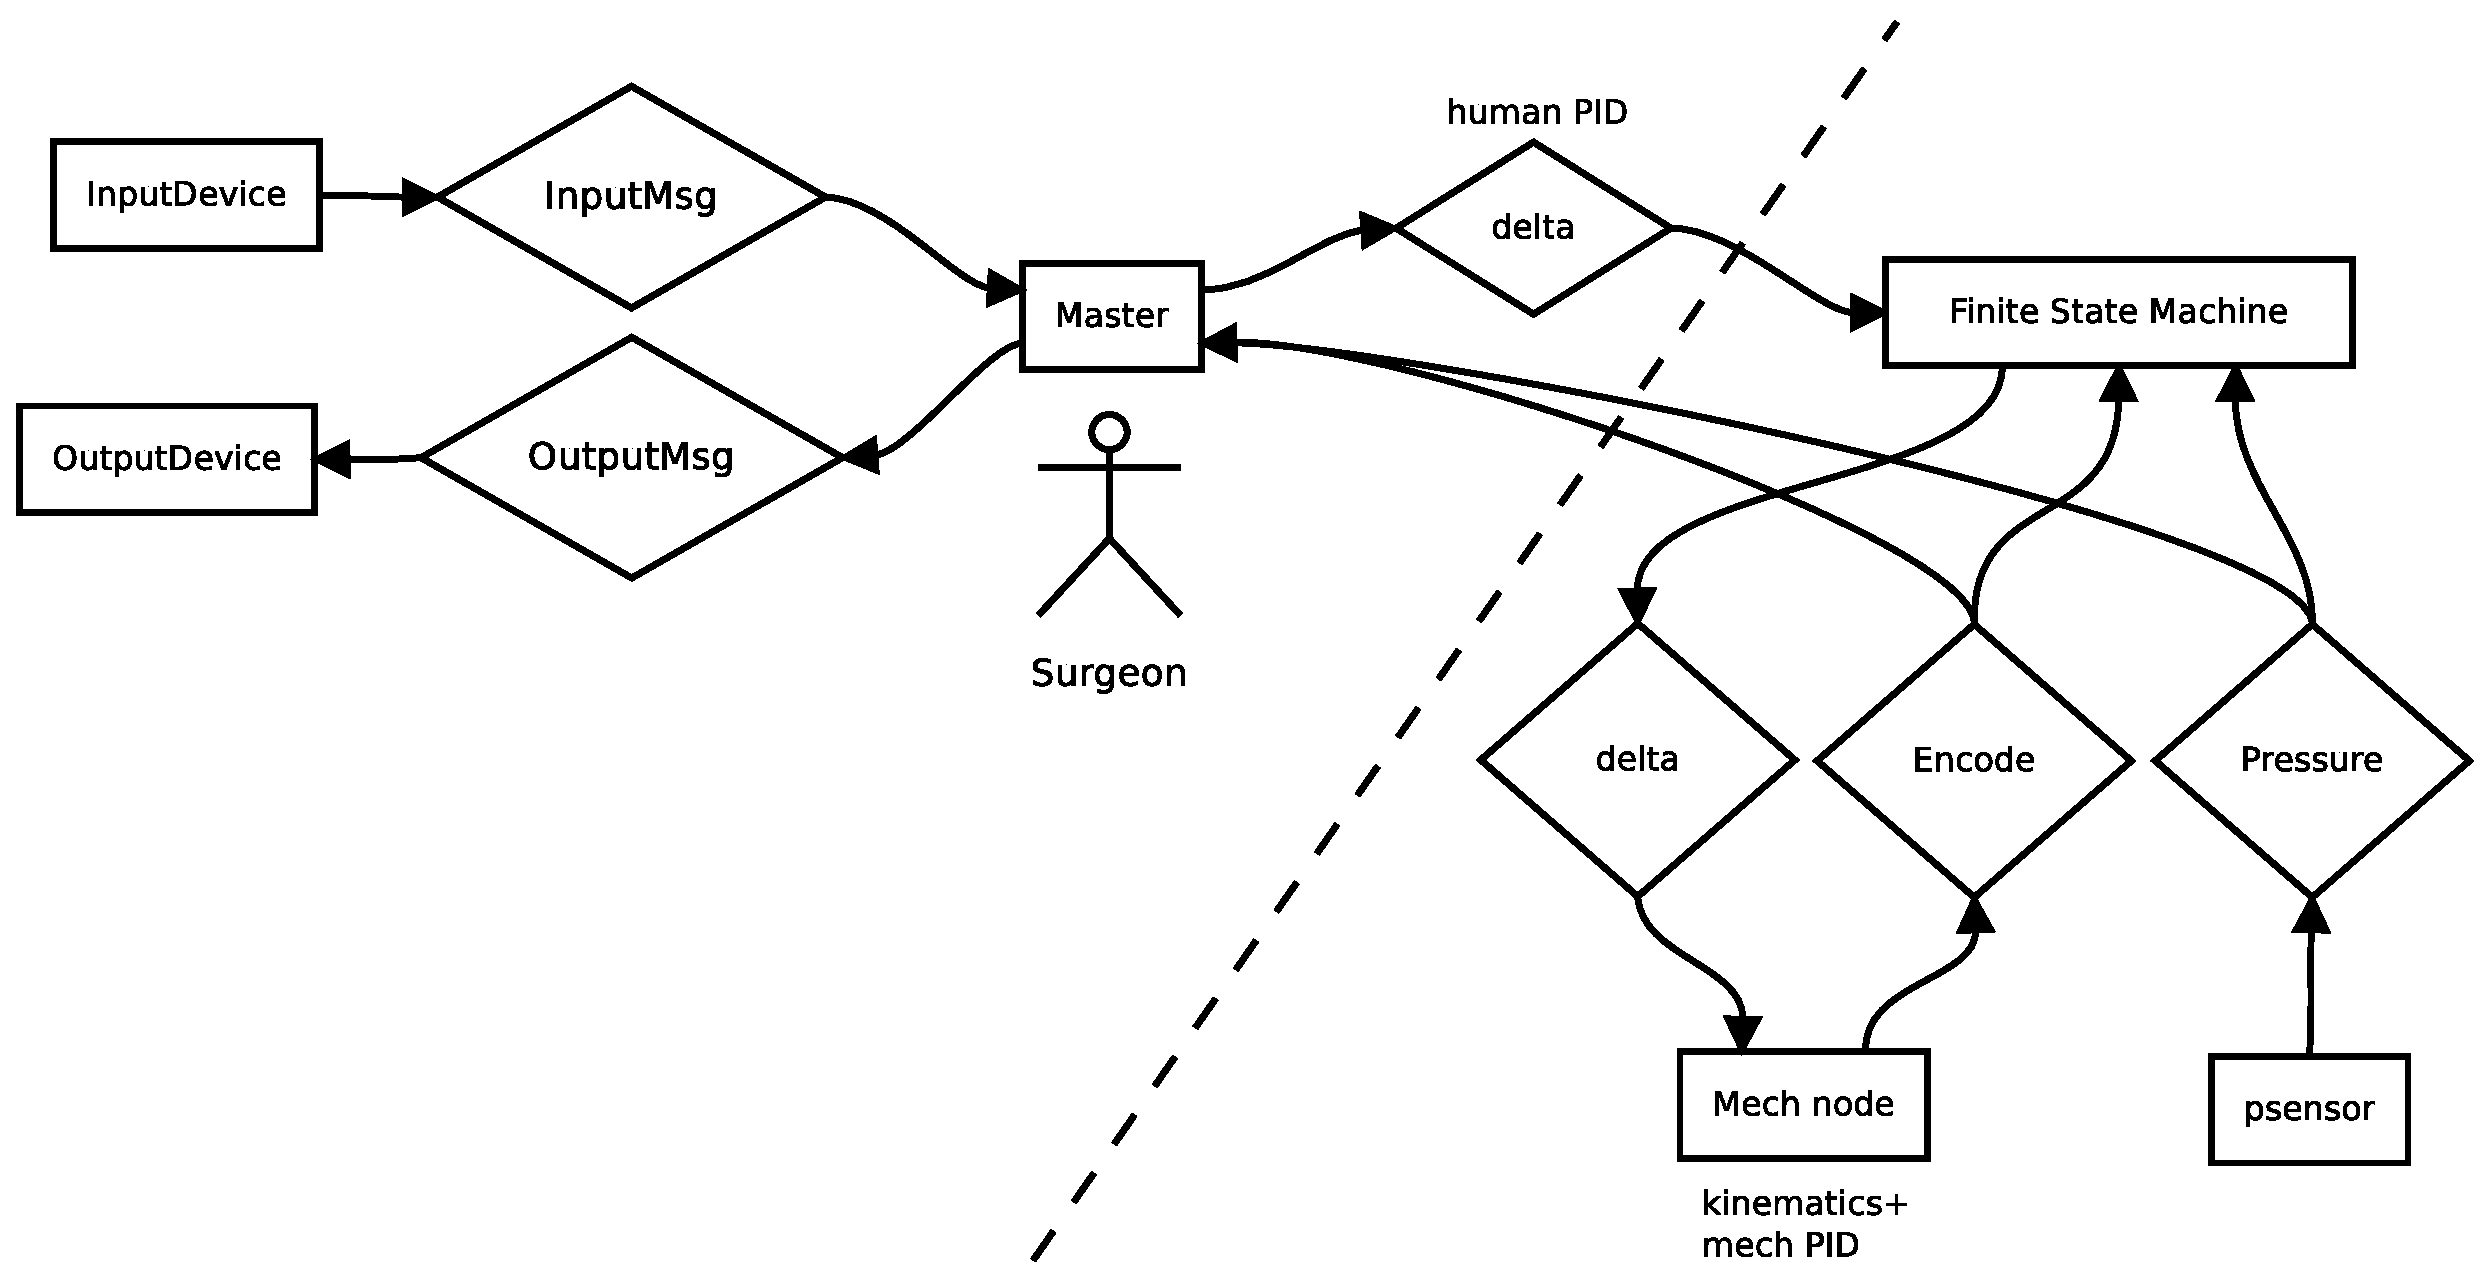
\includegraphics[width=1.0\textwidth]{ros_high_level_v2.eps}
  \end{center}
  \caption{Proposed ROS network for the Raven II. Everything to the
    left of the dashed line is \emph{master}, and everything to the
    right is \emph{slave}. Squares represent ROS nodes, diamonds
    represent ROS topics for passing messages.}
  \label{fig:ros_network}
\end{figure*}

Our top-level design of the ROS network replaces the \emph{networking}
thread, \emph{console I/O} thread, and the entire master side with ROS
components. The square Mech node in Figure~\ref{fig:ros_network}
encasulates most of the existing raven code, including all of the code
responsible for gravity compensation, inverse kinematics, PID control,
and USB I/O. Our ROS network defines a standard interface between the
InputDevice node and the Master node, which would make implementing
new input devices straightforward---adding Wii Remote support or
LapaRobot support to the Raven should be straightforward since it
would not require knowledge of any part of the ROS network beyond its
interface with the Master node.

\subsection{Master: Generic Control}

BRL hard-coded the control side as part of the Raven-II system so that
the control device can only be the Sensable Phantom Omni. Although the
Phantom Omni is a widely used haptic device for medical simulation and
training [2], such constraint would be a limiting factor for projects
involving other types of controllers. In our reimplementation, the
control node is contained within an independent ROS package called
{\it raven\_control}. It interacts with the finite state machine in
{\it raven\_fsm} through the ROS messaging system, as shown in Figure
1.

\begin{figure}[h]
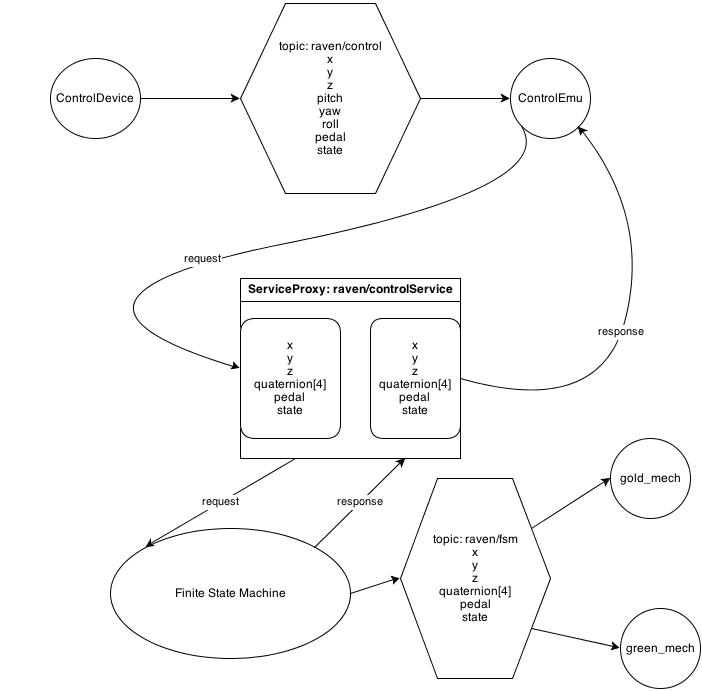
\includegraphics[scale=0.33]{ControlDiagram.jpg}
\caption{Controller-FSM Messaging}
\end{figure}

The {\it ControlDevice} node indicates the actual control device from
the user end. When the user triggers a control event, {\it
  ControlDevice} publishes the message (x, y, z, pitch, yaw, roll,
pedal and state) to the topic {\it raven/control}. On the subscriber
end, {\it ControlEmu} transforms the values of pitch, yaw and roll
into quaternion required by {\it raven\_mech}. The communication
between {\it ControlEmu} and the finite state machine is established
through a ROS service\footnote{ROS Services,
  http://www.ros.org/wiki/Services}. {\it ControlEmu} sends a request
to the service proxy which the finite state machine (FSM in short)
listens to. Once a control request is received, the FSM formulates a
message object and sends it to the topic {\it raven/fsm} subscribed by
the arm nodes (the arms are labeled "green" and "gold
respectively"). Once the arms are ready for next control event, the
FSM evaluates the situation and accordingly sends back a response to
{\it ControlEmu}. {\it ControlEmu} then issues a new request based on
the previous response.

Compared to the BRL's implementation, our implementation allows
generic control devices besides the Phantom Omni. The tested working
devices are keyboards, PlayStation3 controllers and generic PC game
controllers. Due to the incompleteness of the development, a control
device node needs to be manually added following the template in
Figure 2.

\begin{figure}[h]
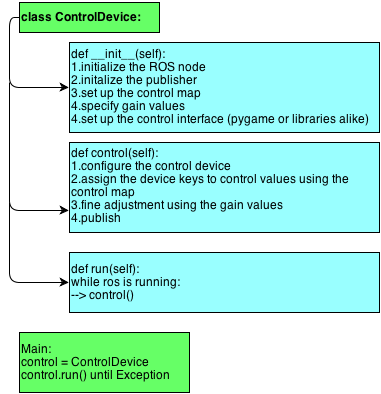
\includegraphics[scale=0.6]{ControlDeviceTemplate.png}
\caption{Control Device Python Template}
\end{figure}

Eventually users will be able to add and configure control devices
through either a {\it control.xml} file or a GTK
interface\footnote{GTK,http://www.gtk.org/}. The proper control nodes
will be generated based on the user input.

\subsection{Slave: Finite State Machine}

The finite state machine serves as a high-level commander of the
Raven-II system. It's in charge of the state estimation and
transition. Figure 3 shows the work flow of the FSM.

\begin{figure}[h]
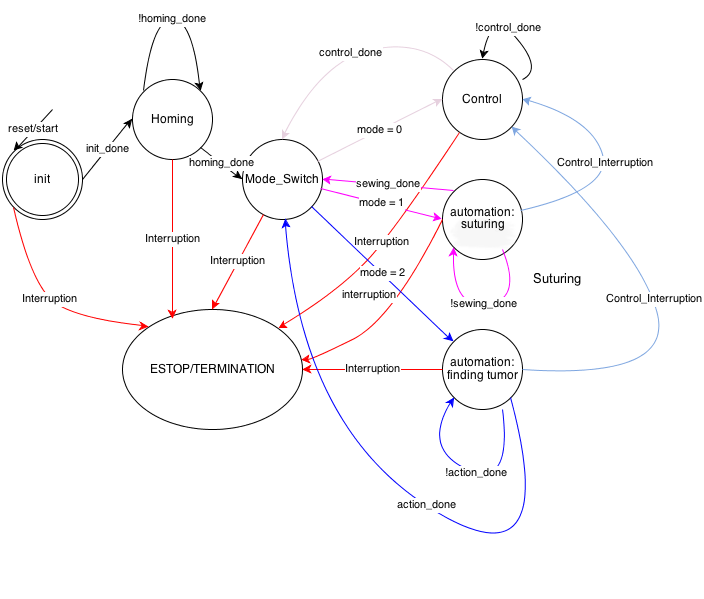
\includegraphics[scale=0.4]{FSM.png}
\caption{FSM Work Flow}
\end{figure}

After initialization, the FSM starts inspecting {\it raven\_mech}'s
homing action until it's done. The "Mode\_Switch" state is where major
estimation and transitions happen. Based on the user input, the FSM
transits to the corresponding state (control, sewing automation, tumor
tracking, etc). The current implementation leaves room for more modes
in the future development. Among all the modes, "Control" has the
highest priority. Any other modes can be interrupted by the user
control. This is a rather naive implementation mainly for testing and
is subject to change. Among all the states, "ESTOP/TERMINATION" has
the highest priority. The FSM goes to this state once there is an
emergency interruption. The FSM would then save the current state
record and properly stop the Raven-II system. The FSM is also designed
to communicate with external ROS nodes. Essentially modes can hand
work to ROS nodes and collect status for progress through
services. One example is the controller-FSM messaging mentioned in the
"Generic Control" section. If the "Control" mode is active, the FSM
communicates with {\it ControlEmu} through a service, gives {\it
  raven\_mech} orders through messages and reports to "Mode\_Switch"
for state estimation.

\subsection{Slave: Mech} % How do you move this so that it's after the figure??

\subsection{Message Format Between Master and Slave}
- Pedal up/down

- Position

- Quaternions

\section{Mistakes}

\section{Conclusion}


%% {\footnotesize \bibliographystyle{acm}
%% \bibliography{../common/bibliography}}

%% \theendnotes

\end{document}
